\lecture{4}{3/2}

\begin{example}[DOC middleware]
    \hfill
    \begin{enumerate}
        \item 
            Java RMI and Python Pyro closely follow traditional
            development processes basing themselves on library
            integration and parameter passing.

        \item 
            COBRA is similar to Java RMI and Pyro but it integrates
            components developed using different programming
            languages.
            This allows us to use components regardless on
            the language they were developed in,
            we just need an IDL.
            COBRA allows both asynchronous and synchronous operation
            but is not popular due to it being so complex.
    \end{enumerate}
\end{example}

\section{Message-oriented middleware}

\begin{definition}[Message-oriented middleware]
    \textbf{Message-oriented middleware} (MOM) is a software
    and hardware infrastructure that supports sending and receiving 
    messages between distributed systems.
\end{definition}

\begin{figure}[]
    \centering
    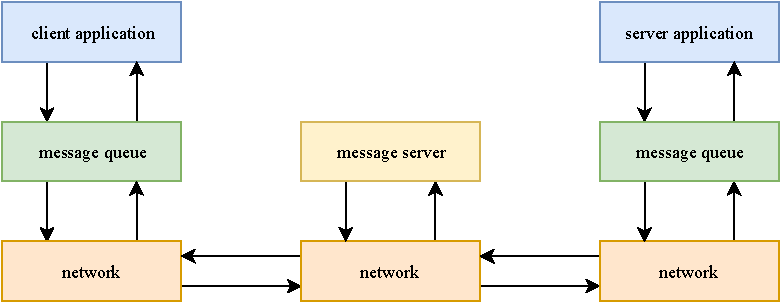
\includegraphics[width=0.8\linewidth]{images/mom.pdf}
    \caption{
        A diagram demonstrating how message-oriented middleware
        operates.
    }
    \label{fig:mom}
\end{figure}

\begin{remark}
    There is a question of why complicate communications with
    a third-party message server?
    If a server crashes, the message server can hold messages
    until it comes back online.
    Additionally,
    we can reduce redudancy on requests.
    If a server has many identical requests, the message server
    can reduce this down to one request.
    It can also act as a filter; implementing features such as priority.
\end{remark}

\paragraph{Properities of MOM}
\begin{enumerate}
    \item It can facilitate of asychronous communication;
    \item It is a reliable delivery service.
    \item It can implement filtering, logging, and data transformations.
    \item It is a natural implementation for database integration.
\end{enumerate}

\begin{example}
    Java Message Service (JMS) is an example of  MOM.
\end{example}

\chapter{Web services}

\begin{definition}[Web service]
    A web service (WS) is a server serving web documents
    (such as XML, JSON, HTML, etc.)
    and creating WS apps over web protocols (HTTPS).
\end{definition}

For communications, web services may use XML to express message
contents via the \textbf{simple object access protocol} (SOAP)
(this is a lightweight protocol for communication).
We describe how web services should be used using a 
\textbf{web services description language} (WSDL) and, as a client,
we \emph{discover} web services through a \emph{UDDI registry}.

\begin{figure}[]
    \centering
    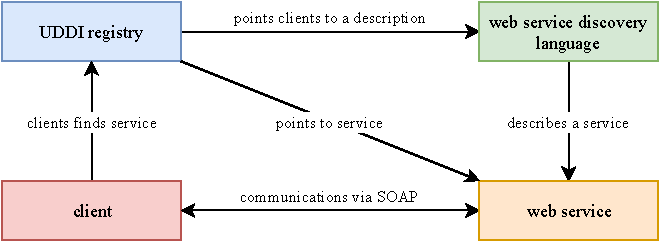
\includegraphics[width=0.8\linewidth]{images/web-services.pdf}
    \caption{
        A diagram illustrating the process of a client connecting
        to a web service via a UDDI registry.
    }
    \label{fig:web-services}
\end{figure}

The client must contact a UDDI registry to get the description of
the web service \emph{and} find the physical location of the server.

XML and JSON are both markup languages used in communications in
distributed systems; however,
JSON is easier to read and use.

\begin{example}[XML vs JSON]
    \hfill
    \begin{center}
        \ttfamily
        \begin{tabular}{lp{1em}l}
            \toprule
            XML && JSON \\
            \midrule
            <?xml version = '1'> && 
            \{ \\
            <auth-context> && \hspace{1em} 
            'username': 'benapier'
            \\
            \hspace{1em} <username> benapier &&
            \} \\
            \hspace{1em} </username> \\
            </auth-context> \\
            \bottomrule
        \end{tabular}
    \end{center}
    Both of these examples convey the same amount of information.
\end{example}

\begin{example}
    REST is a URL interface for accessing resources.
    For example, the URL
    \begin{center}
        \ttfamily
        https://github.com/benapier
    \end{center}
    will access the profile of the username \texttt{benapier}.
\end{example}

\begin{example}[AWS]
    Amazon web services (AWS) are a collection of remote computing services.
    They provide a barebones experience in distributing systems.
\end{example}

\begin{example}[Google WS]
    Google web services are similar to AWS, but is more application oriented
    allowing use of sophisticated APIs.
\end{example}
